\documentclass[xcolor=dvipsnames]{beamer}
\usepackage[T1]{fontenc}
\usepackage[utf8]{inputenc}
\usepackage[english,slovak]{babel}

\usepackage{amsmath}
\usepackage{amsthm}
\usetheme{Pittsburgh}
\useoutertheme{shadow}

\usepackage{graphicx}
\usepackage{caption}
\usepackage{subcaption}

\usepackage[]{algorithm2e}
\usepackage{listings}
 \setbeamercovered{transparent}
 \usepackage{cuted}
\usepackage[export]{adjustbox}
\usepackage{mathtools}

\usepackage{lipsum}
\usepackage{verbatim}
\usepackage{transparent}
\usepackage{framed}
\usepackage{xcolor}

\usepackage{multirow}
\usepackage{colortbl}
\usepackage{lmodern}

\usepackage{movie15}
\usepackage{media9}
\usepackage{verbatim}

\usepackage{animate}


\usepackage{hyperref}

\newcommand\Wider[2][3em]{%
\makebox[\linewidth][c]{%
  \begin{minipage}{\dimexpr\textwidth+#1\relax}
  \raggedright#2
  \end{minipage}%
  }%
}






\iftrue

\usetheme{Warsaw}

\setbeamercolor{normal text}{fg=white,bg=black!90}
\setbeamercolor{structure}{fg=white}

\setbeamercolor{alerted text}{fg=red!85!black}

\setbeamercolor{item projected}{use=item,fg=black,bg=item.fg!35}

\setbeamercolor*{palette primary}{use=structure,fg=structure.fg}
\setbeamercolor*{palette secondary}{use=structure,fg=structure.fg!95!black}
\setbeamercolor*{palette tertiary}{use=structure,fg=structure.fg!90!black}
\setbeamercolor*{palette quaternary}{use=structure,fg=structure.fg!95!black,bg=black!80}

\setbeamercolor*{framesubtitle}{fg=white}

\setbeamercolor*{block title}{parent=structure,bg=black!60}
\setbeamercolor*{block body}{fg=black,bg=black!10}
\setbeamercolor*{block title alerted}{parent=alerted text,bg=black!15}
\setbeamercolor*{block title example}{parent=example text,bg=black!15}

\fi



%-------------------------------------------------------------------------------------
\title{\color{white} \bf random network distillation}
\author{\color{white} Michal CHOVANEC, PhD}


%\setbeamertemplate{footline}[frame number]{}
\setbeamertemplate{navigation symbols}{}


\date[EURP]{}
\begin{document}

{
    \usebackgroundtemplate
    {
        \vbox to \paperheight{\vfil\hbox to \paperwidth{\hfil

        {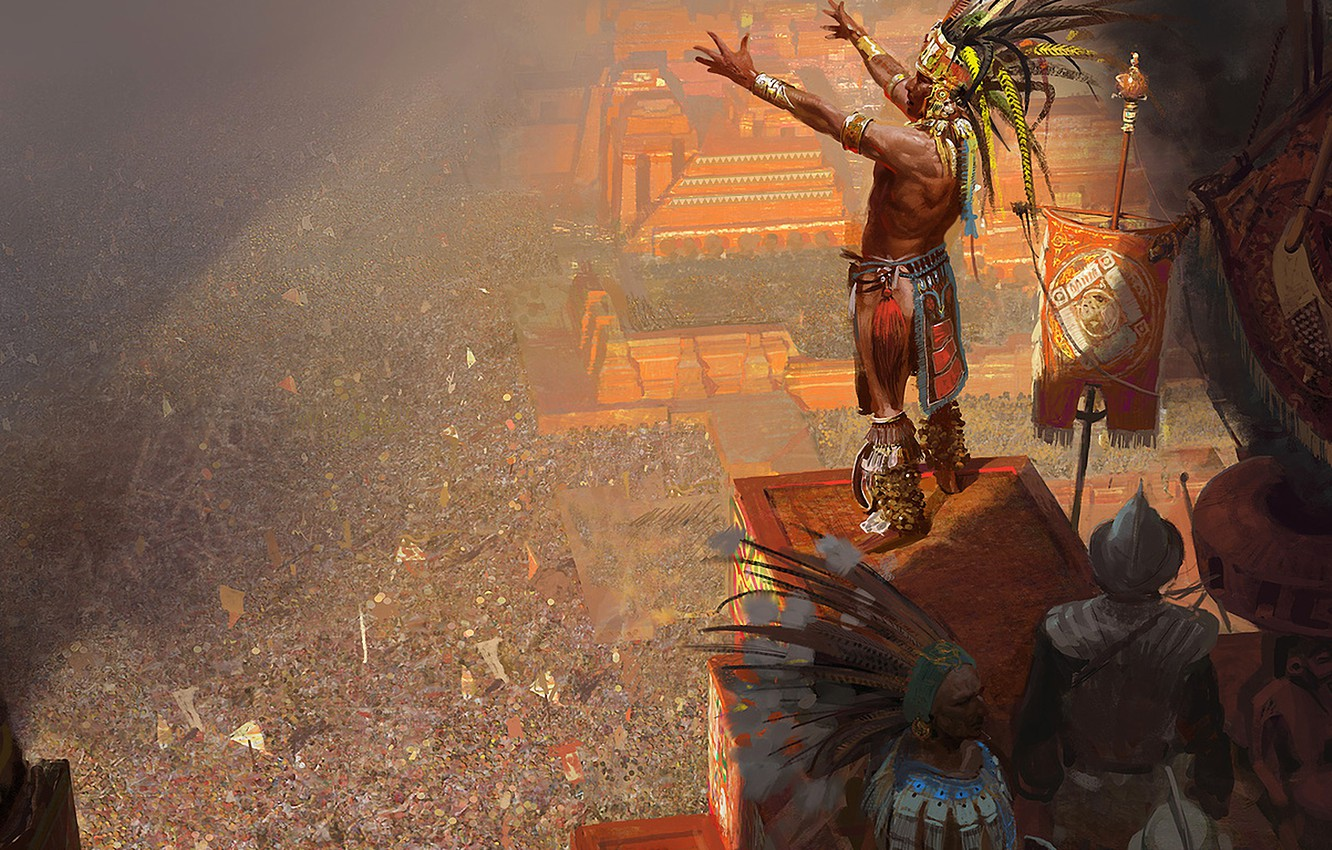
\includegraphics[width=5.05in]{../images/aztec.jpg}}

        \hfil}\vfil}
    }

    \begin{frame}
     \centering
     {
        \begin{minipage}{10cm}
           {\LARGE \color{white}{\bf challenging Montezuma's Revenge}} \\
           {\LARGE \color{white}{\bf intrinsic motivation in RL}} \\
           {\LARGE \color{white}{\bf Michal CHOVANEC}} \\
       \end{minipage}
     }

    \end{frame}
}

\begin{frame}{\bf Montezuma's Revenge}

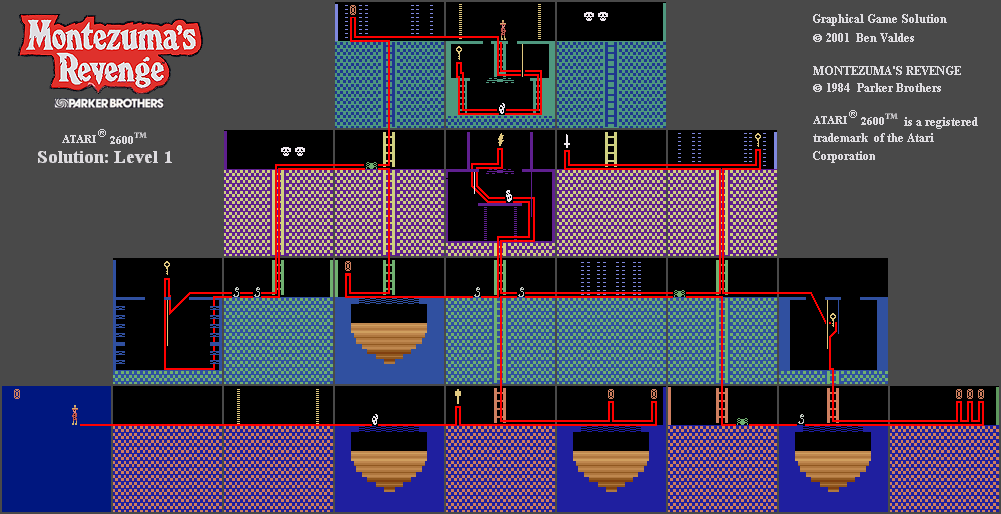
\includegraphics[scale=0.32]{../images/montezuma_map.png}

\end{frame}

\begin{frame}{\bf Montezuma's Revenge}

  \begin{columns}

    \begin{column}{0.5\textwidth}
      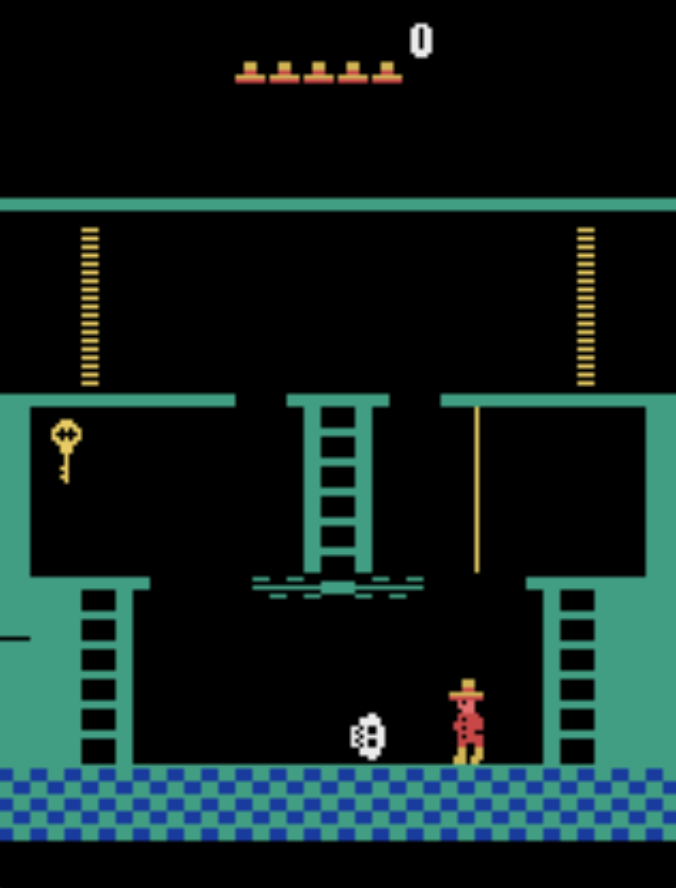
\includegraphics[scale=0.32]{../images/montezuma.png}
    \end{column}

    \begin{column}{0.5\textwidth}
      \begin{itemize}
        \item {\bf very sparse rewards} - hundrets of steps
        \item {\bf huge state space}
        \item {\bf hard exploration}
        \item {\bf needs returns back}
      \end{itemize}
    \end{column}


  \end{columns}

\end{frame}


\begin{frame}{\bf state of the art score}


\begin{columns}
    \column{\dimexpr\paperwidth-10pt}

      source : \url{https://paperswithcode.com/sota/atari-games-on-atari-2600-montezumas-revenge}


      \begin{table}[]
      \begin{tabular}{|l|l|l|}
      \hline
      \textbf{year} & \textbf{name}                                       & \textbf{score} \\ \hline
      2015          & Deep Reinforcement Learning with Double Q-learning  & 0              \\ \hline
      2017          & Curiosity-driven Exploration by Self-supervised Prediction \footnote[1]{https://arxiv.org/abs/1705.05363} & 0       \\ \hline 
      2021          & MuZero                                              & 2500           \\ \hline
      2018          & Count-Based Exploration with Neural Density Models \footnote[2]{https://arxiv.org/abs/1703.01310}  & 3705           \\ \hline
      \textbf{2019} & \textbf{Exploration by Random Network Distillation} \footnote[3]{https://arxiv.org/abs/1810.12894}& \textbf{8152}  \\ \hline
      2021          & GoExplore$^*$ \footnote[4]{https://arxiv.org/abs/2004.12919}                         & 43 000         \\ \hline
      \end{tabular}
      \end{table}

      {\bf * requires environment state saving/loading}

\end{columns}


\end{frame}




\begin{frame}{\bf random network distillation}

\centering
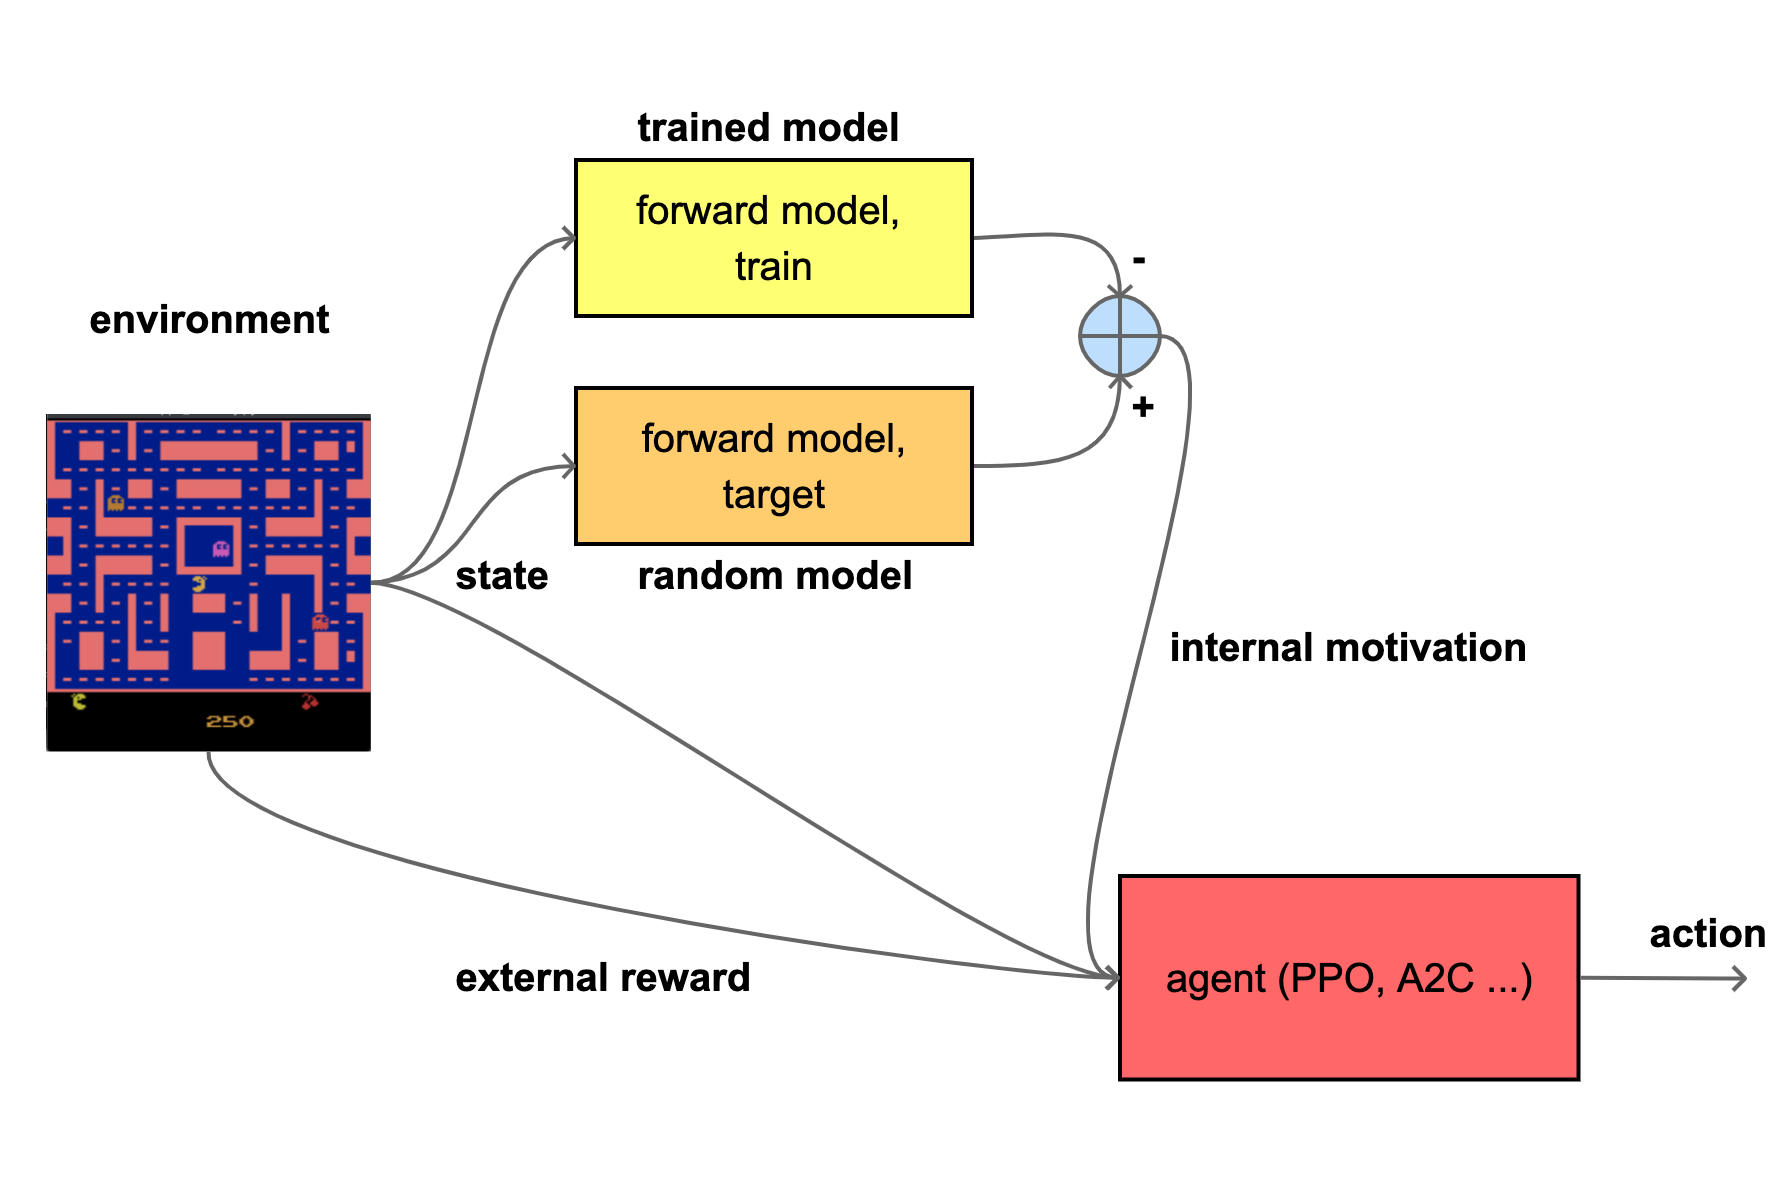
\includegraphics[scale=0.15]{../diagrams/rnd/rnd.png}

\end{frame}

\begin{frame}{\bf random network distillation}

  \begin{columns}

    \begin{column}{0.5\textwidth}
      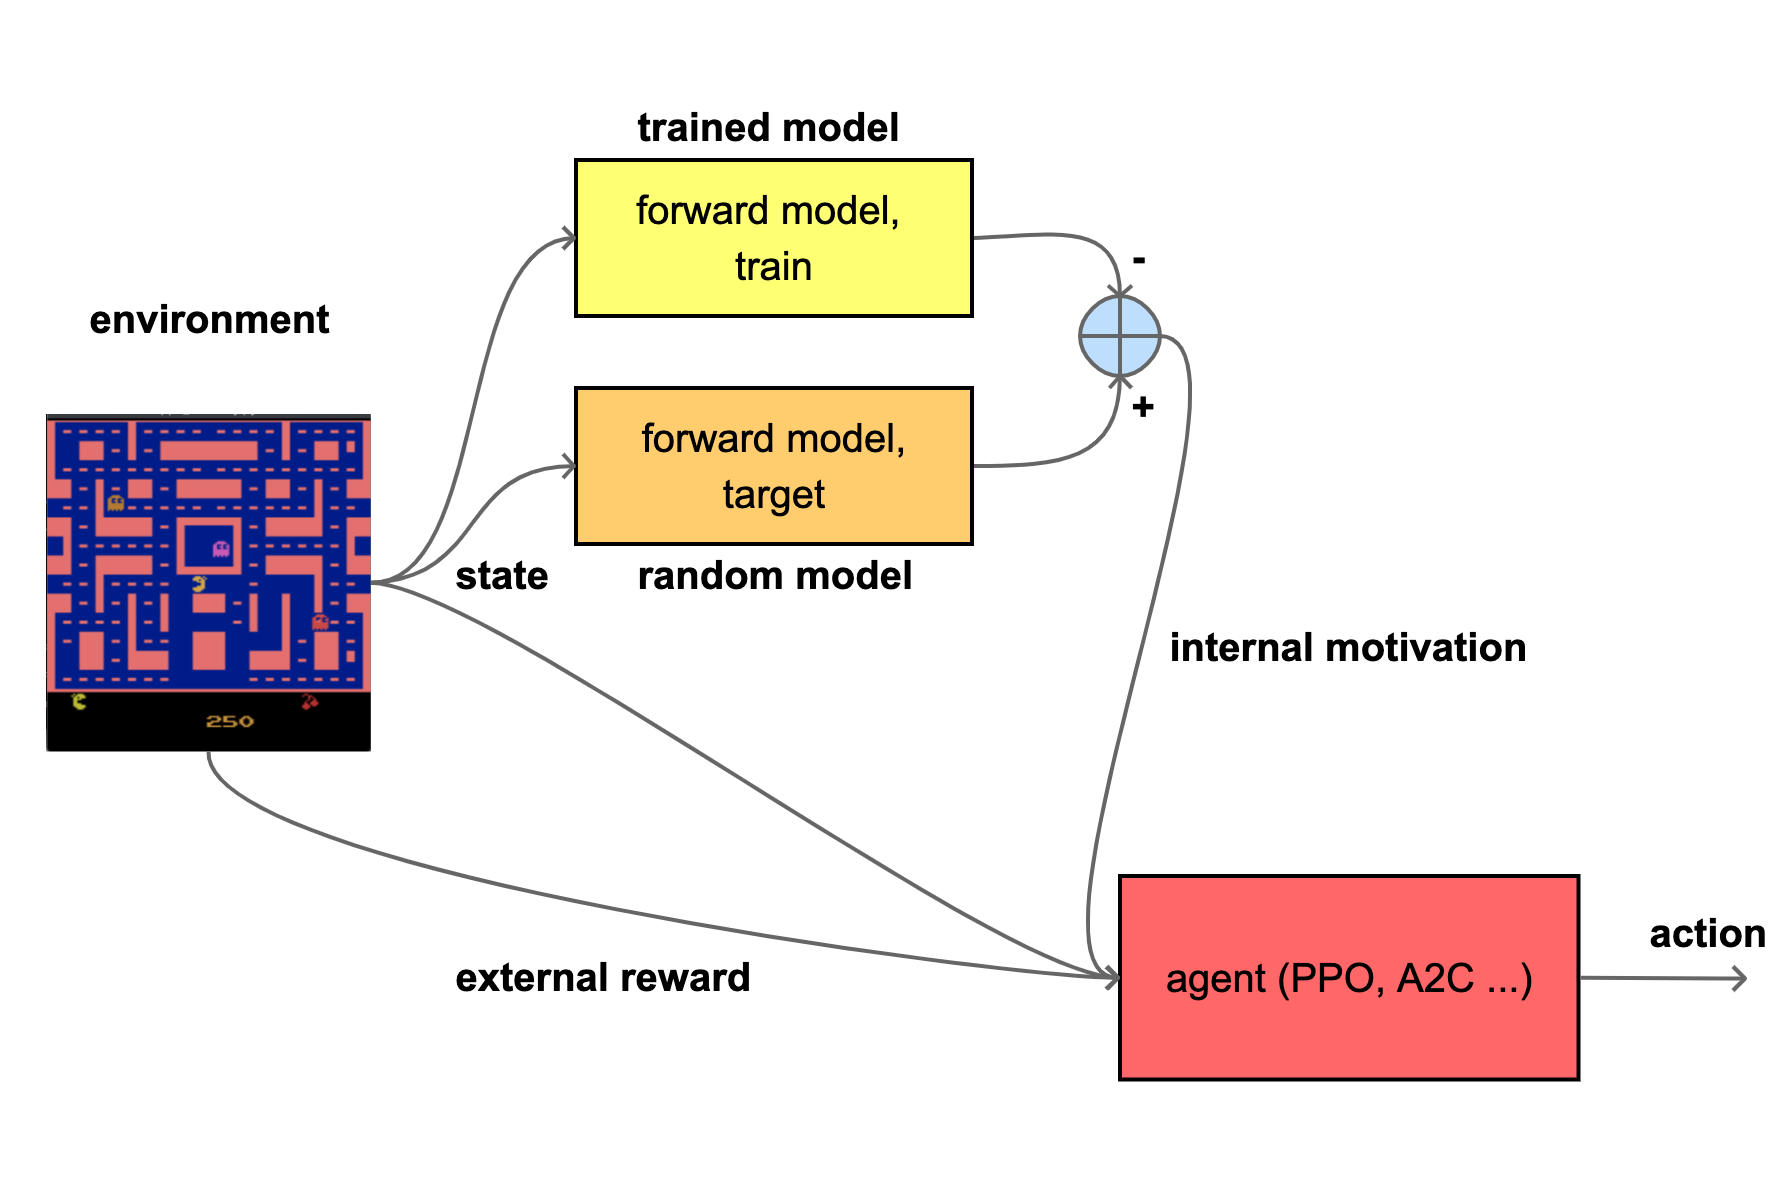
\includegraphics[scale=0.1]{../diagrams/rnd/rnd.png}
    \end{column}

    \begin{column}{0.5\textwidth}
      \begin{itemize}
        \item neural network works as {\bf novelty detector}
        \item model learns to imitate random (target) model
        \item {\bf less visited states produce bigger motivation signal}
        \item orthogonal weights initialisation ($g=2^{0.5}$) for strong signal
        \item lot of fully connected layers {\bf to avoid generalisation}
      \end{itemize}
    \end{column}


  \end{columns}

\end{frame}


\begin{frame}{\bf random network distillation architecture}

\centering
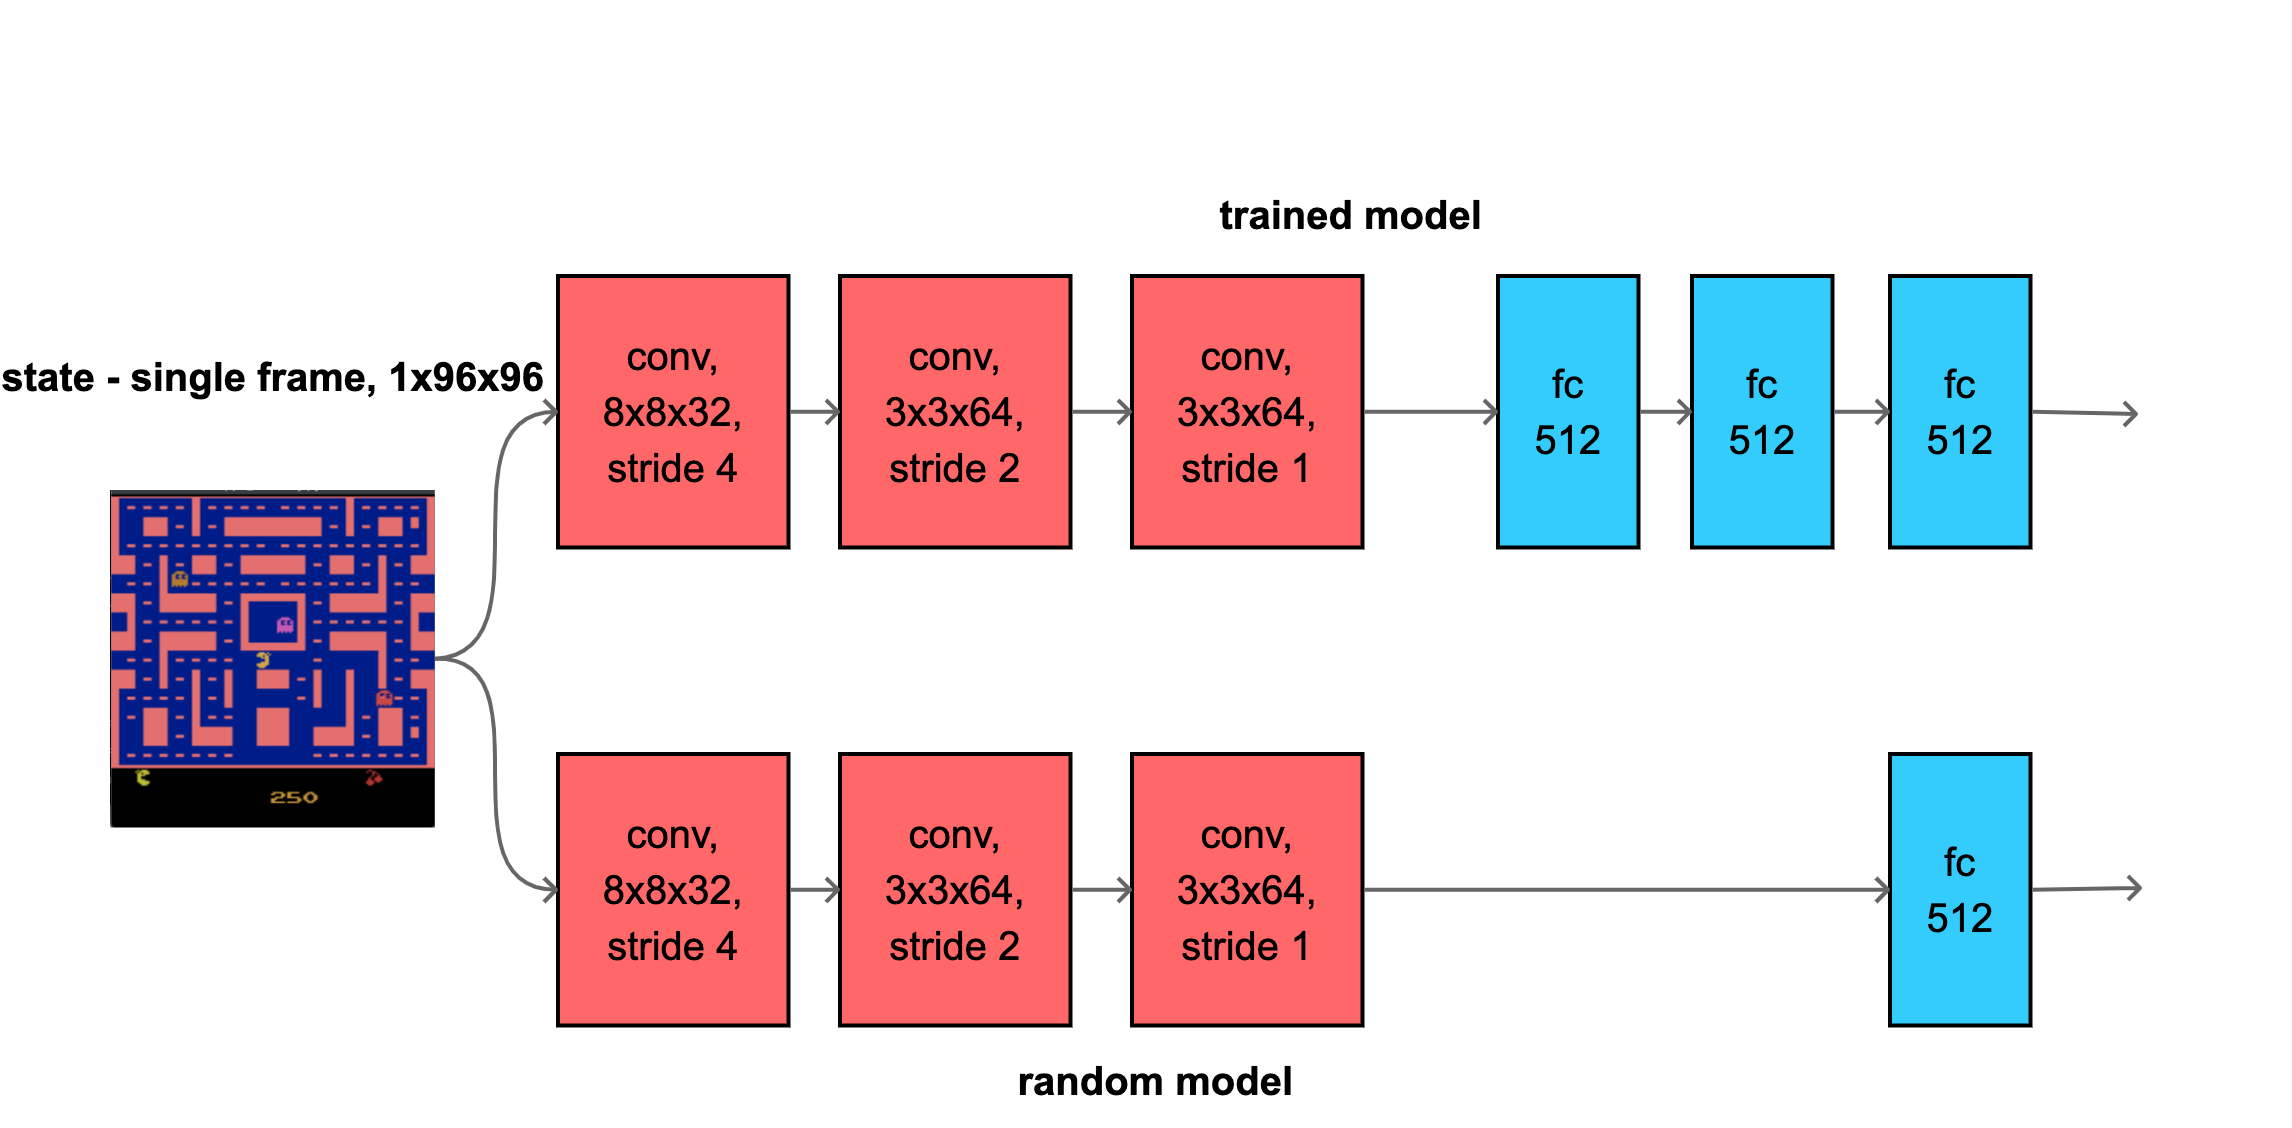
\includegraphics[scale=0.12]{../diagrams/rnd/modelrnd.png}

\end{frame}



\begin{frame}{\bf ppo model architecture}

\centering
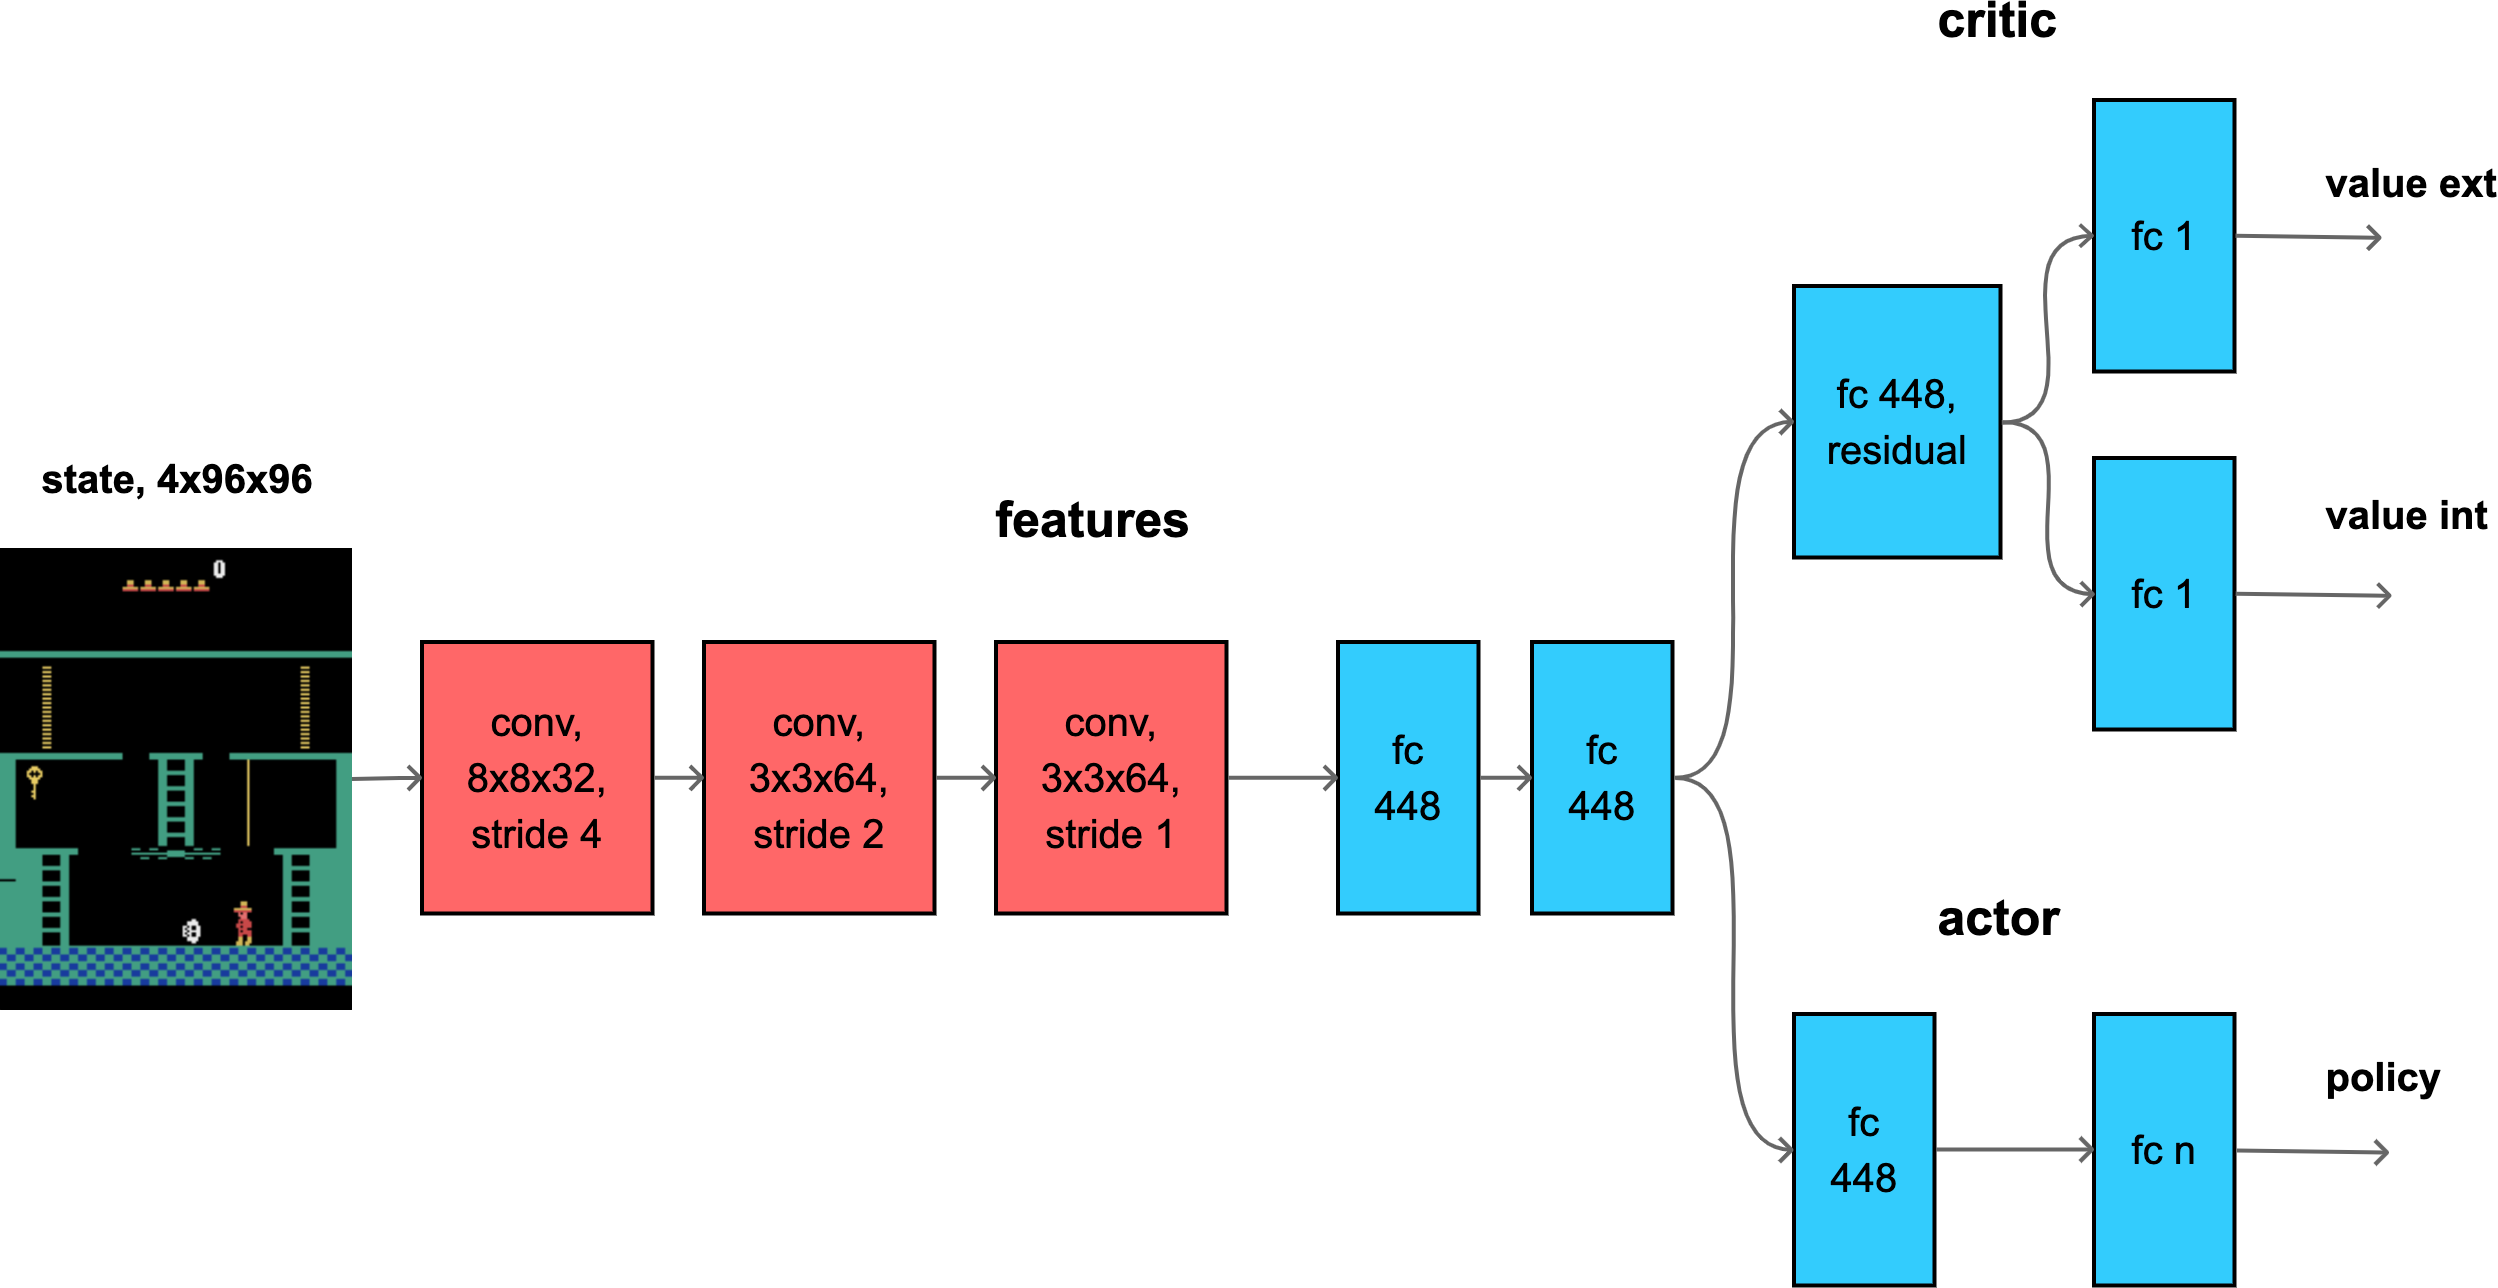
\includegraphics[scale=0.12]{../diagrams/rnd/modelppoa.png}

\end{frame}

\begin{frame}{\bf ppo model architecture}

\centering
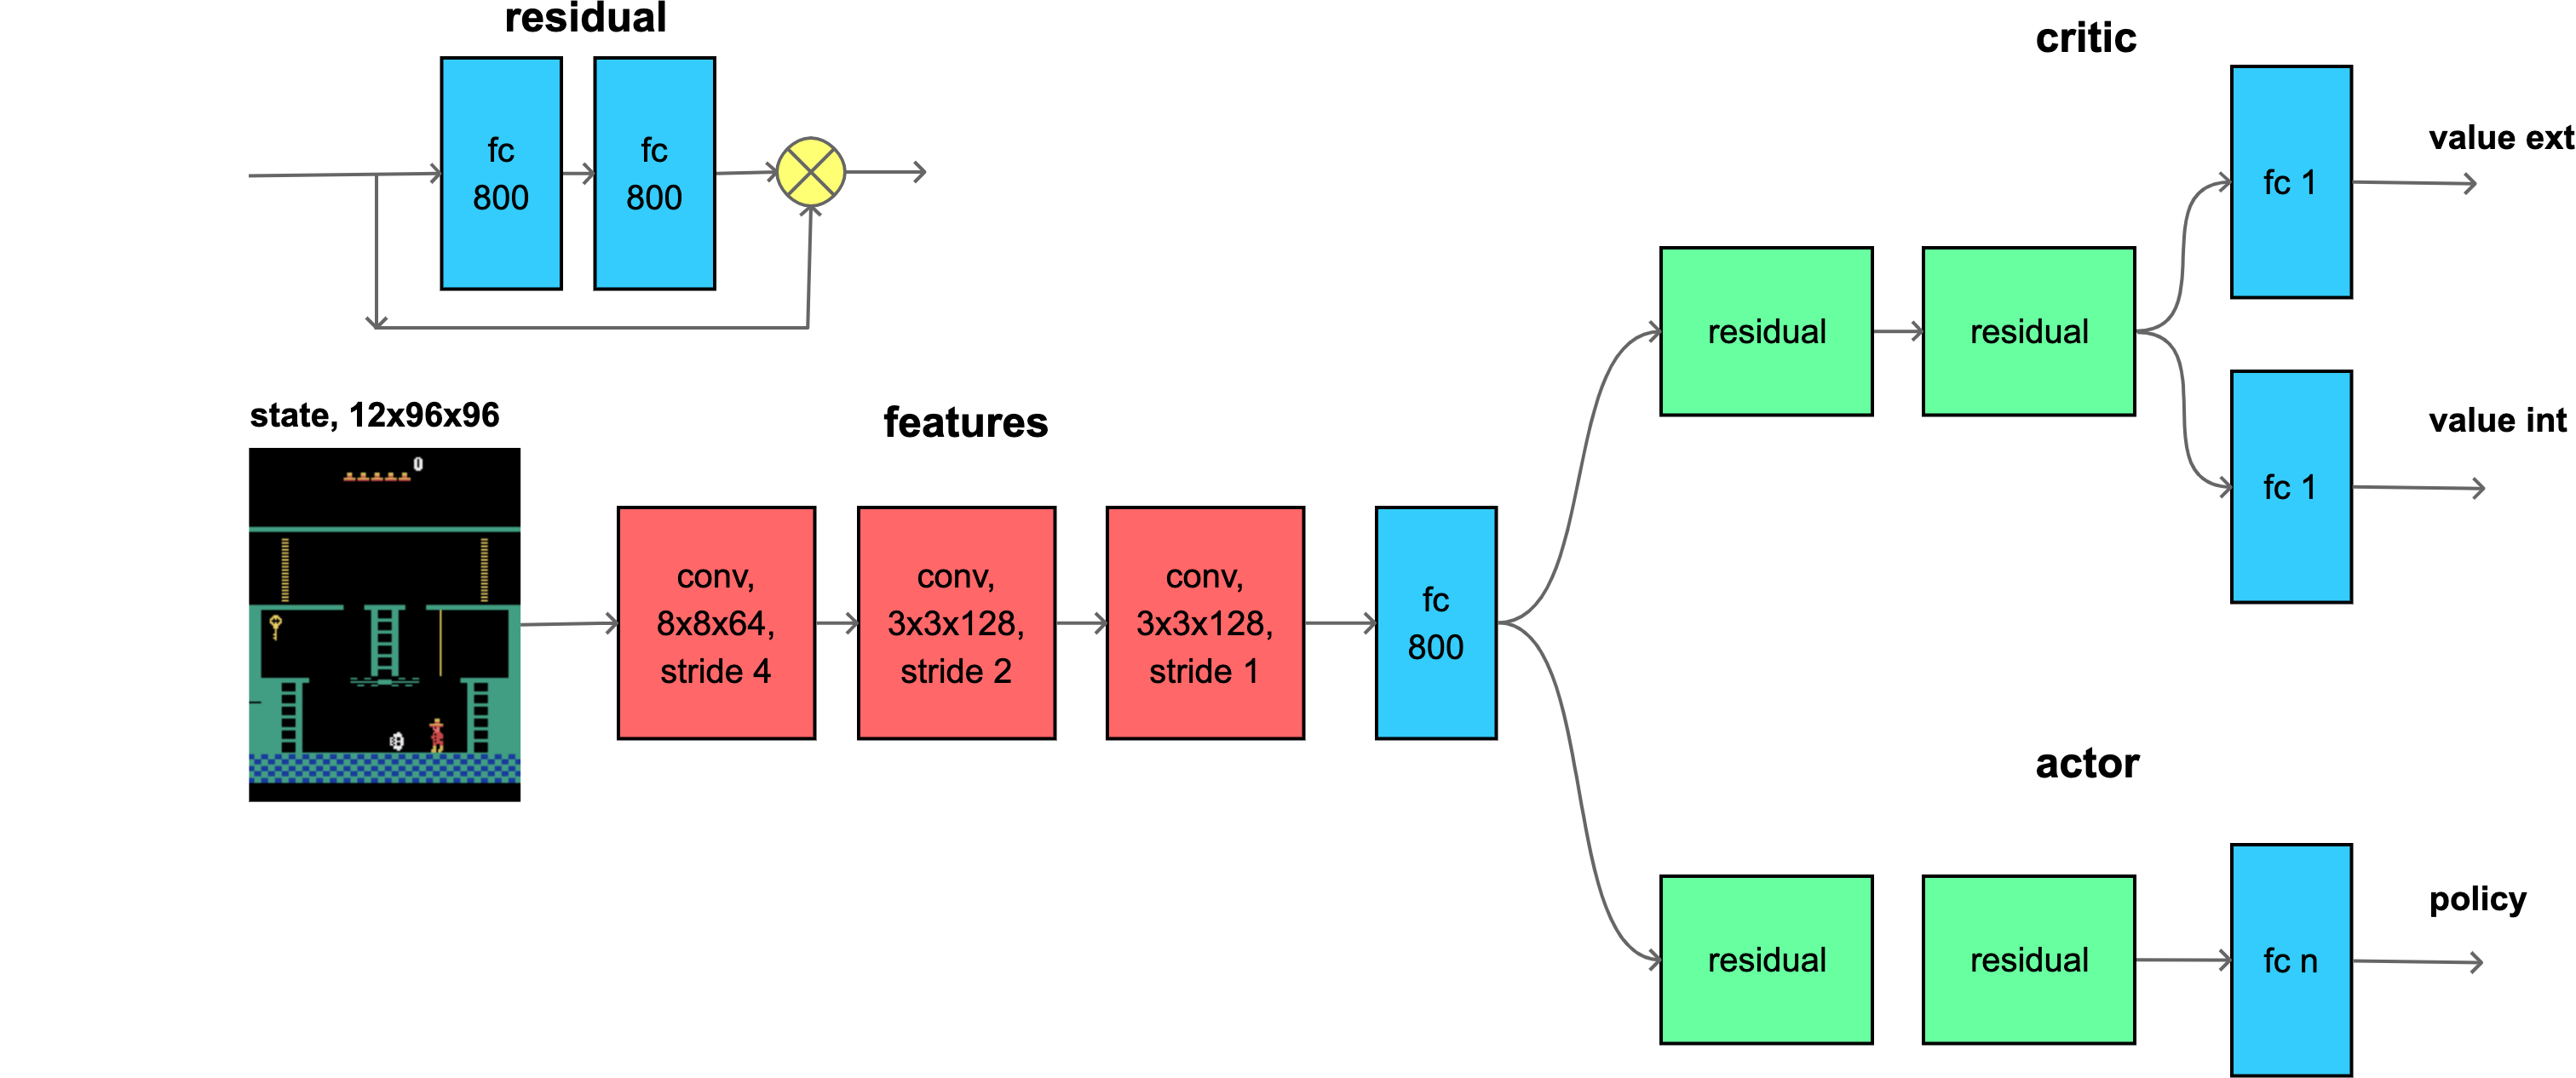
\includegraphics[scale=0.1]{../diagrams/rnd/modelppob.png}

\end{frame}


\begin{frame}{\bf loss}

TODO 

\end{frame}


\begin{frame}{\bf results}


\begin{columns}

    \begin{column}{0.5\textwidth}
      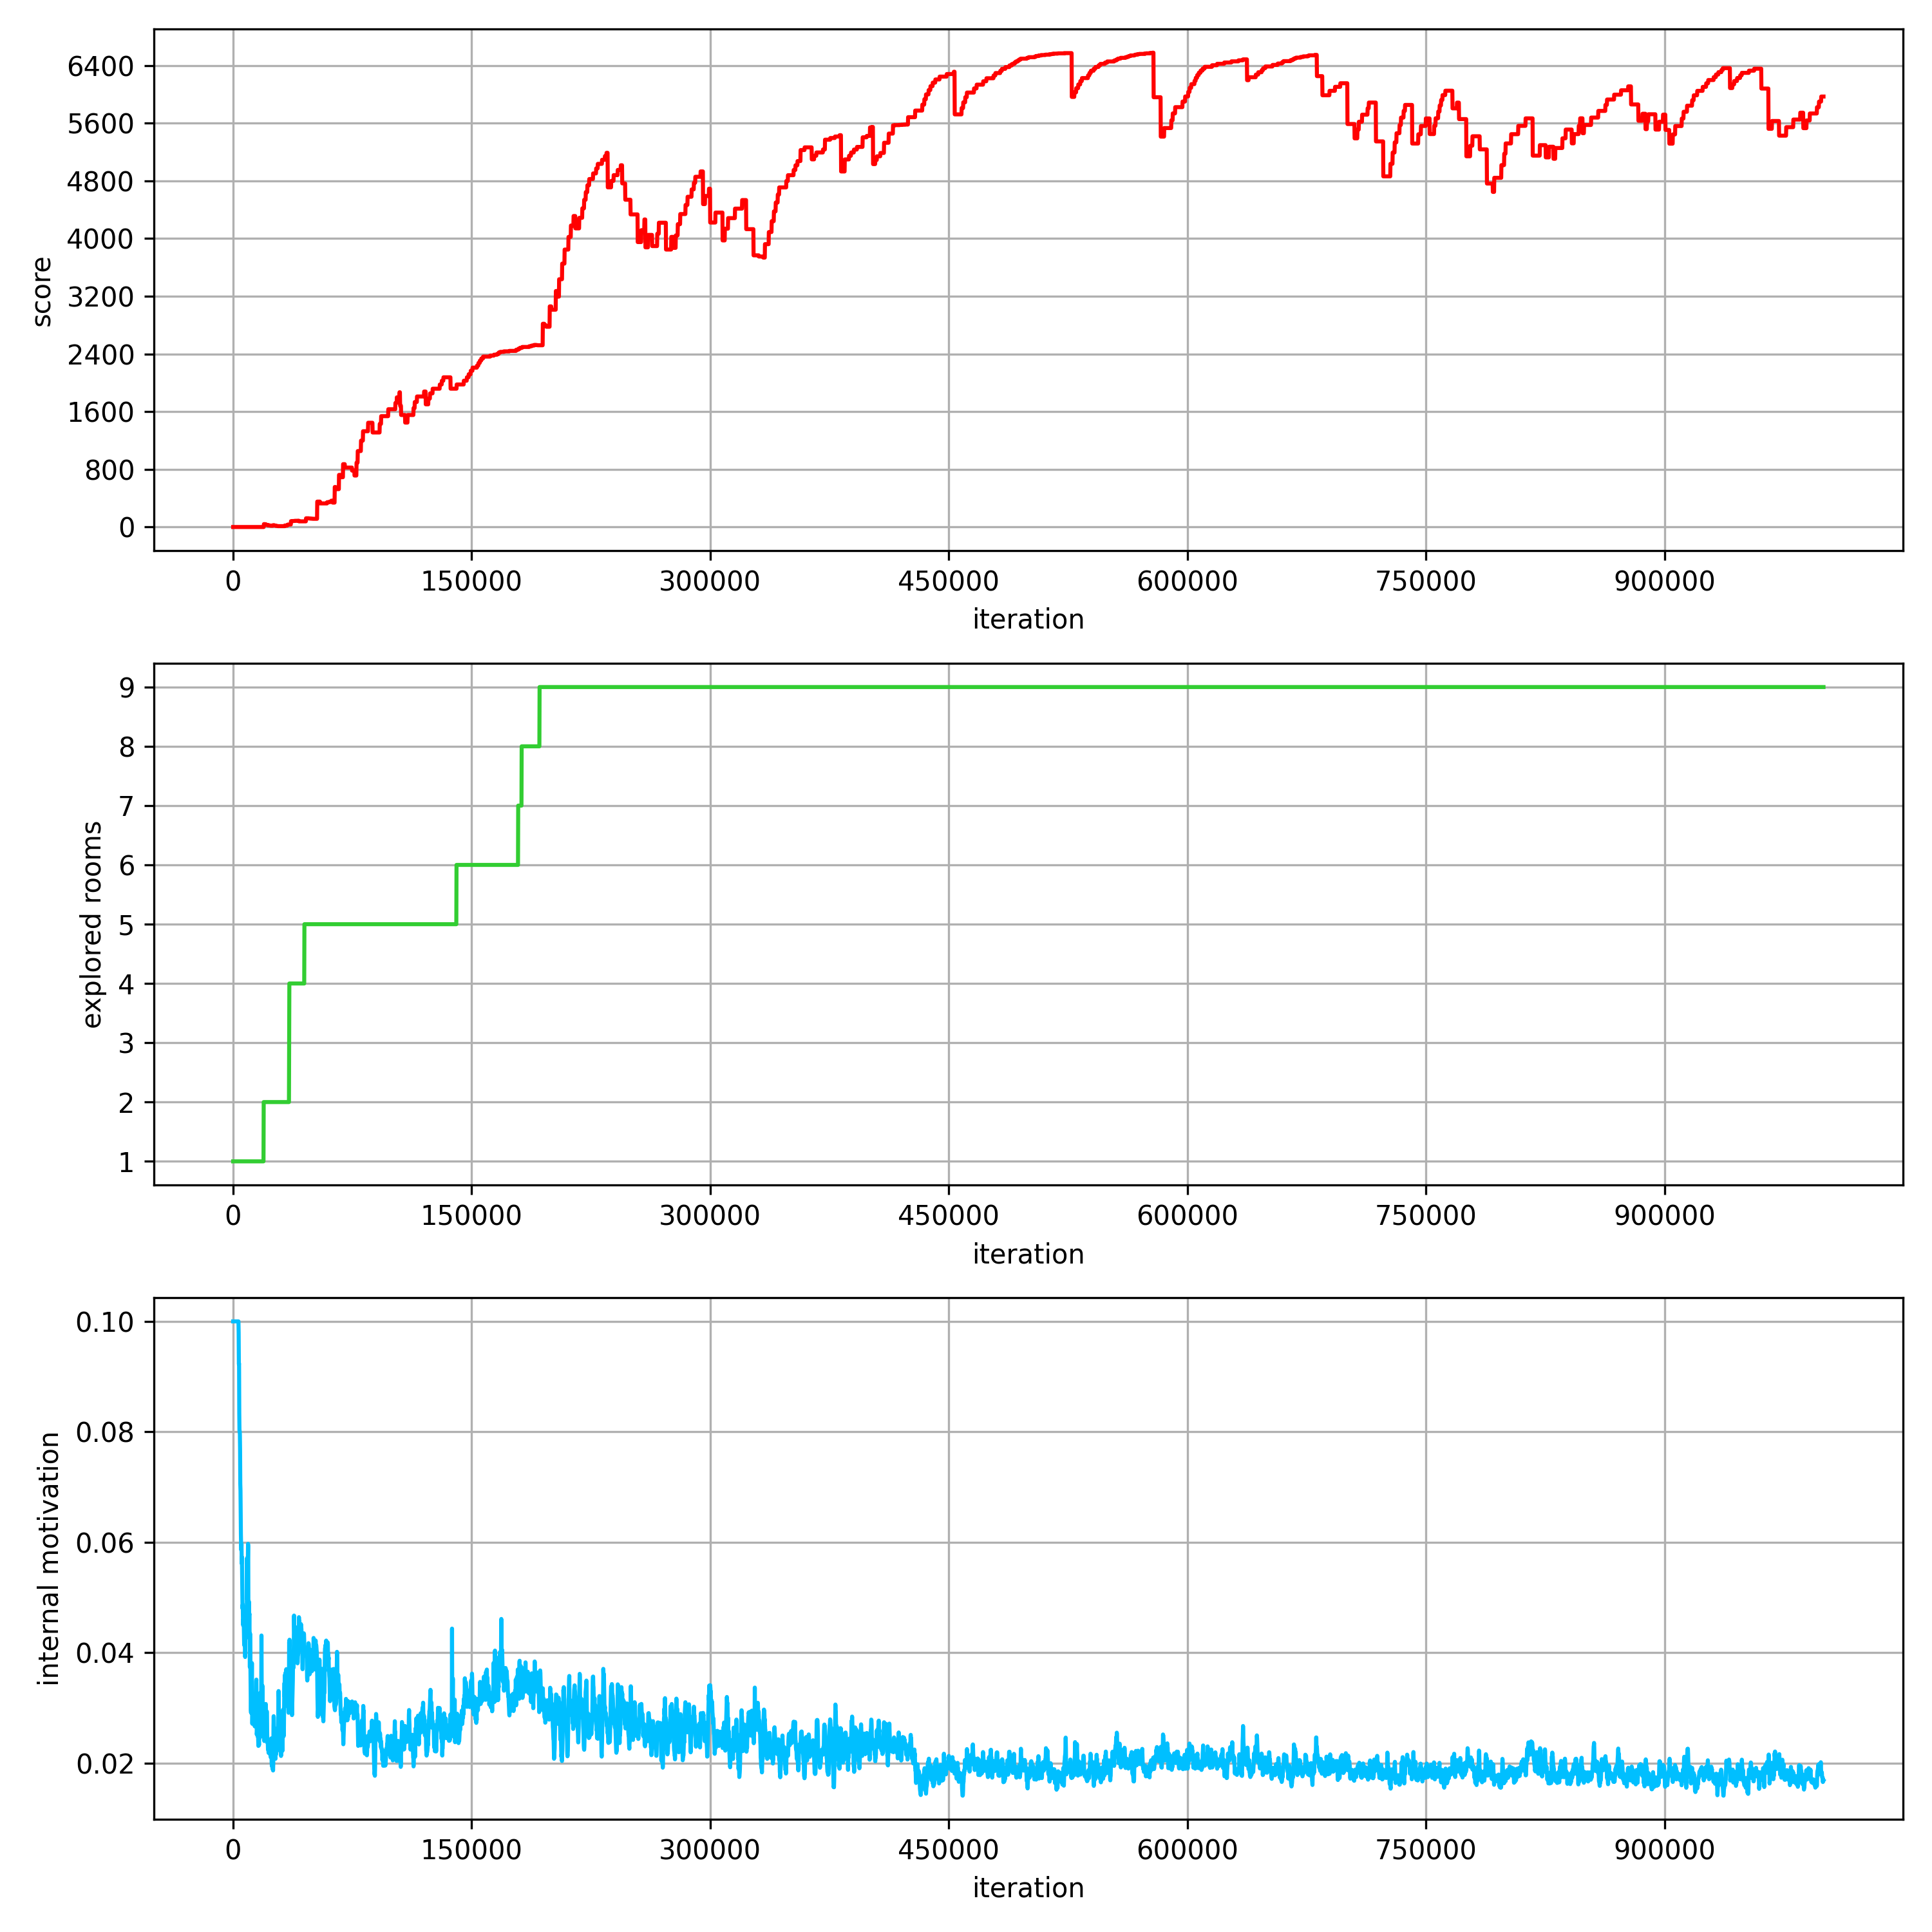
\includegraphics[scale=0.25]{../results/montezuma_ppo_rnd_a.png}
    \end{column}

    \begin{column}{0.5\textwidth}
      \begin{itemize}
        \item 1M  steps - {\bf 20\% of original paper}
        \item 128 parallel envs = total 128M steps
        \item {\bf score 6400}
        \item {\bf 9 rooms explored}
      \end{itemize}
    \end{column}


  \end{columns}


\end{frame}



\begin{frame}{\bf Emergent Tool Use From Multi-Agent Autocurricula}


  \begin{columns}

      \begin{column}{0.5\textwidth}
        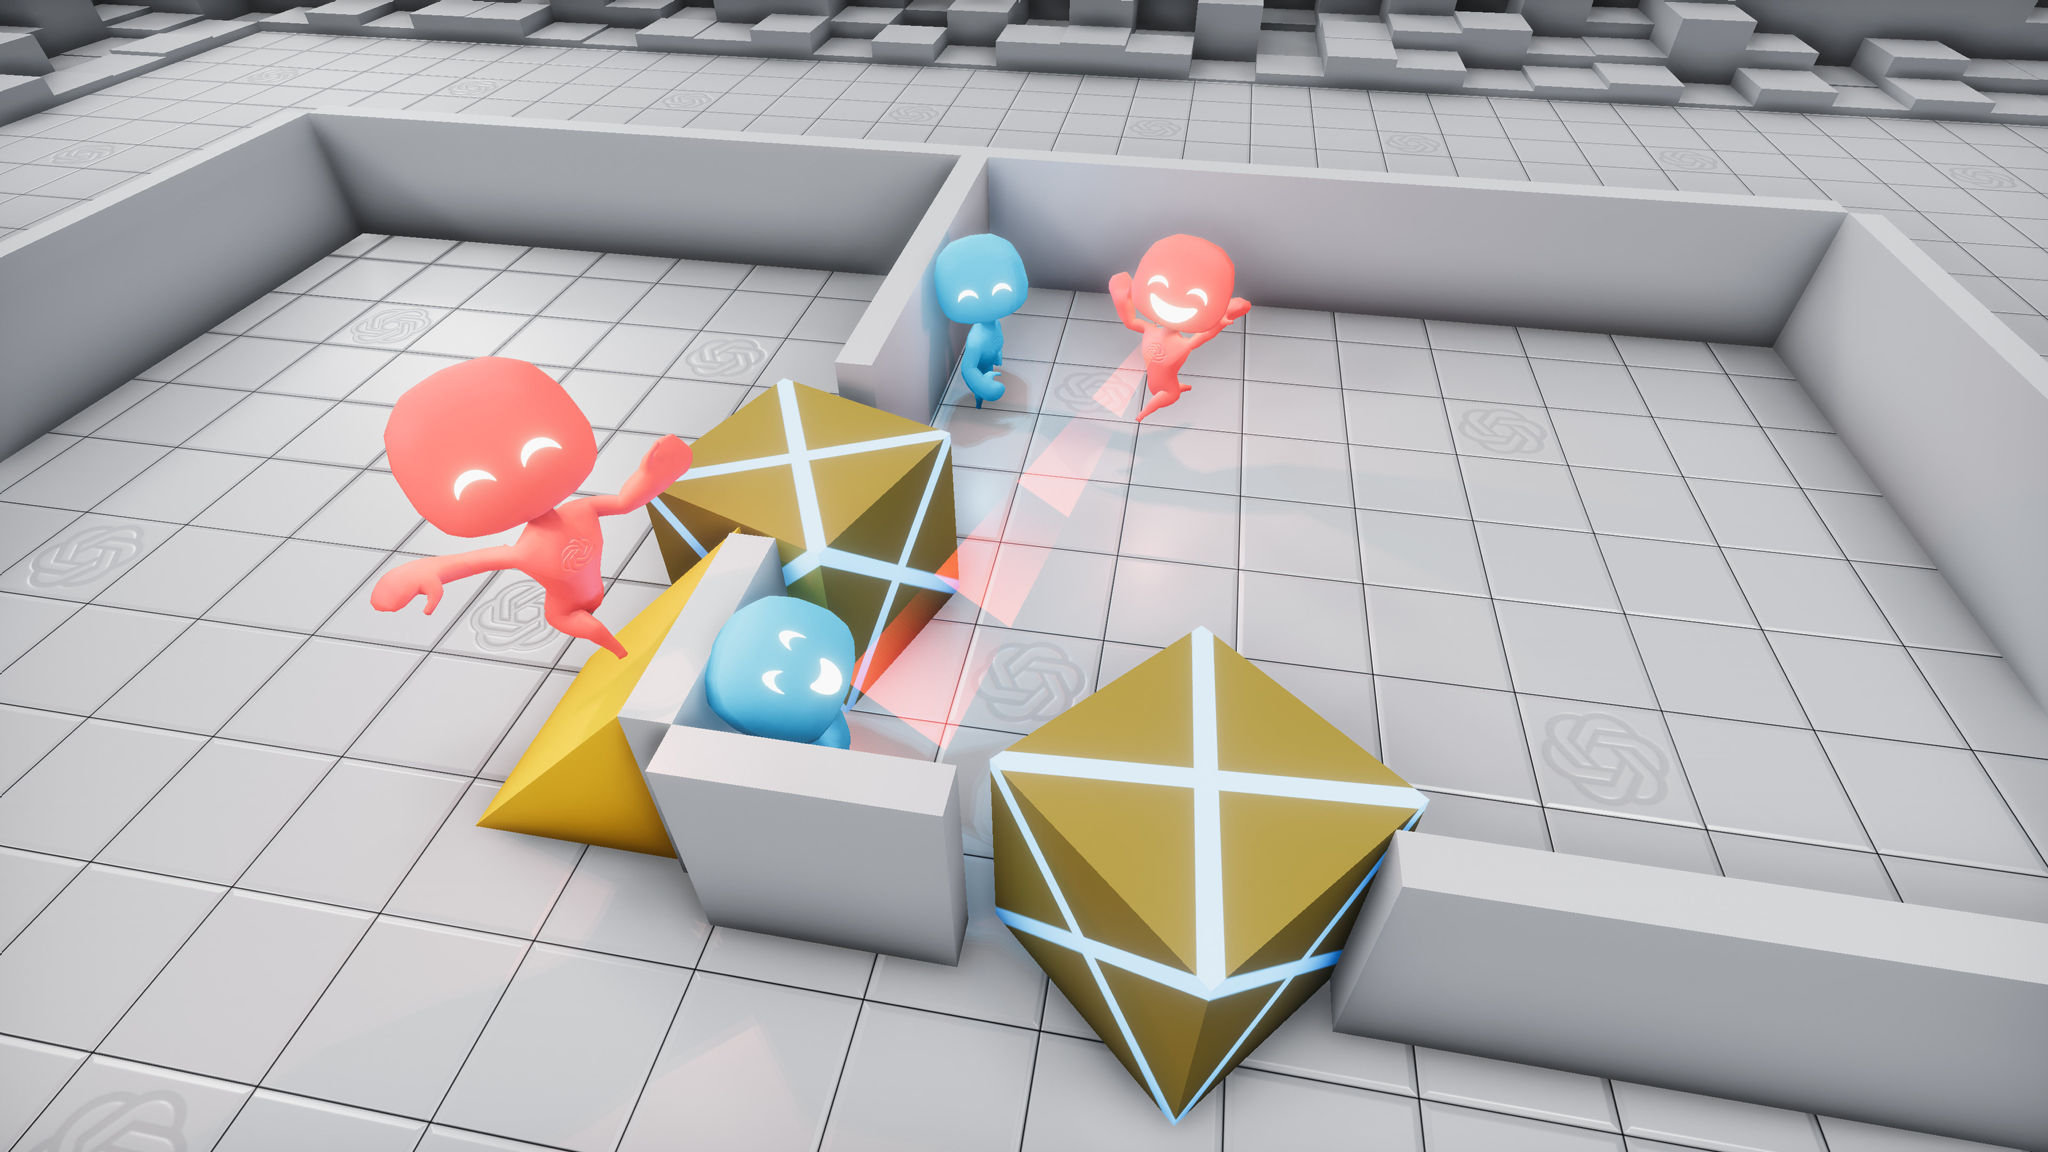
\includegraphics[scale=0.08]{../images/hide_and_seek.jpg}
      \end{column}

      \begin{column}{0.5\textwidth}
        \begin{itemize}
          \item multi-agent robotic environment
          \item hide and seek
          \item \url{https://openai.com/blog/emergent-tool-use/}
          \item \url{https://arxiv.org/abs/1909.07528}
        \end{itemize}
      \end{column}


  \end{columns} 

\end{frame}


\begin{frame}{\bf Q\&A}

\centering{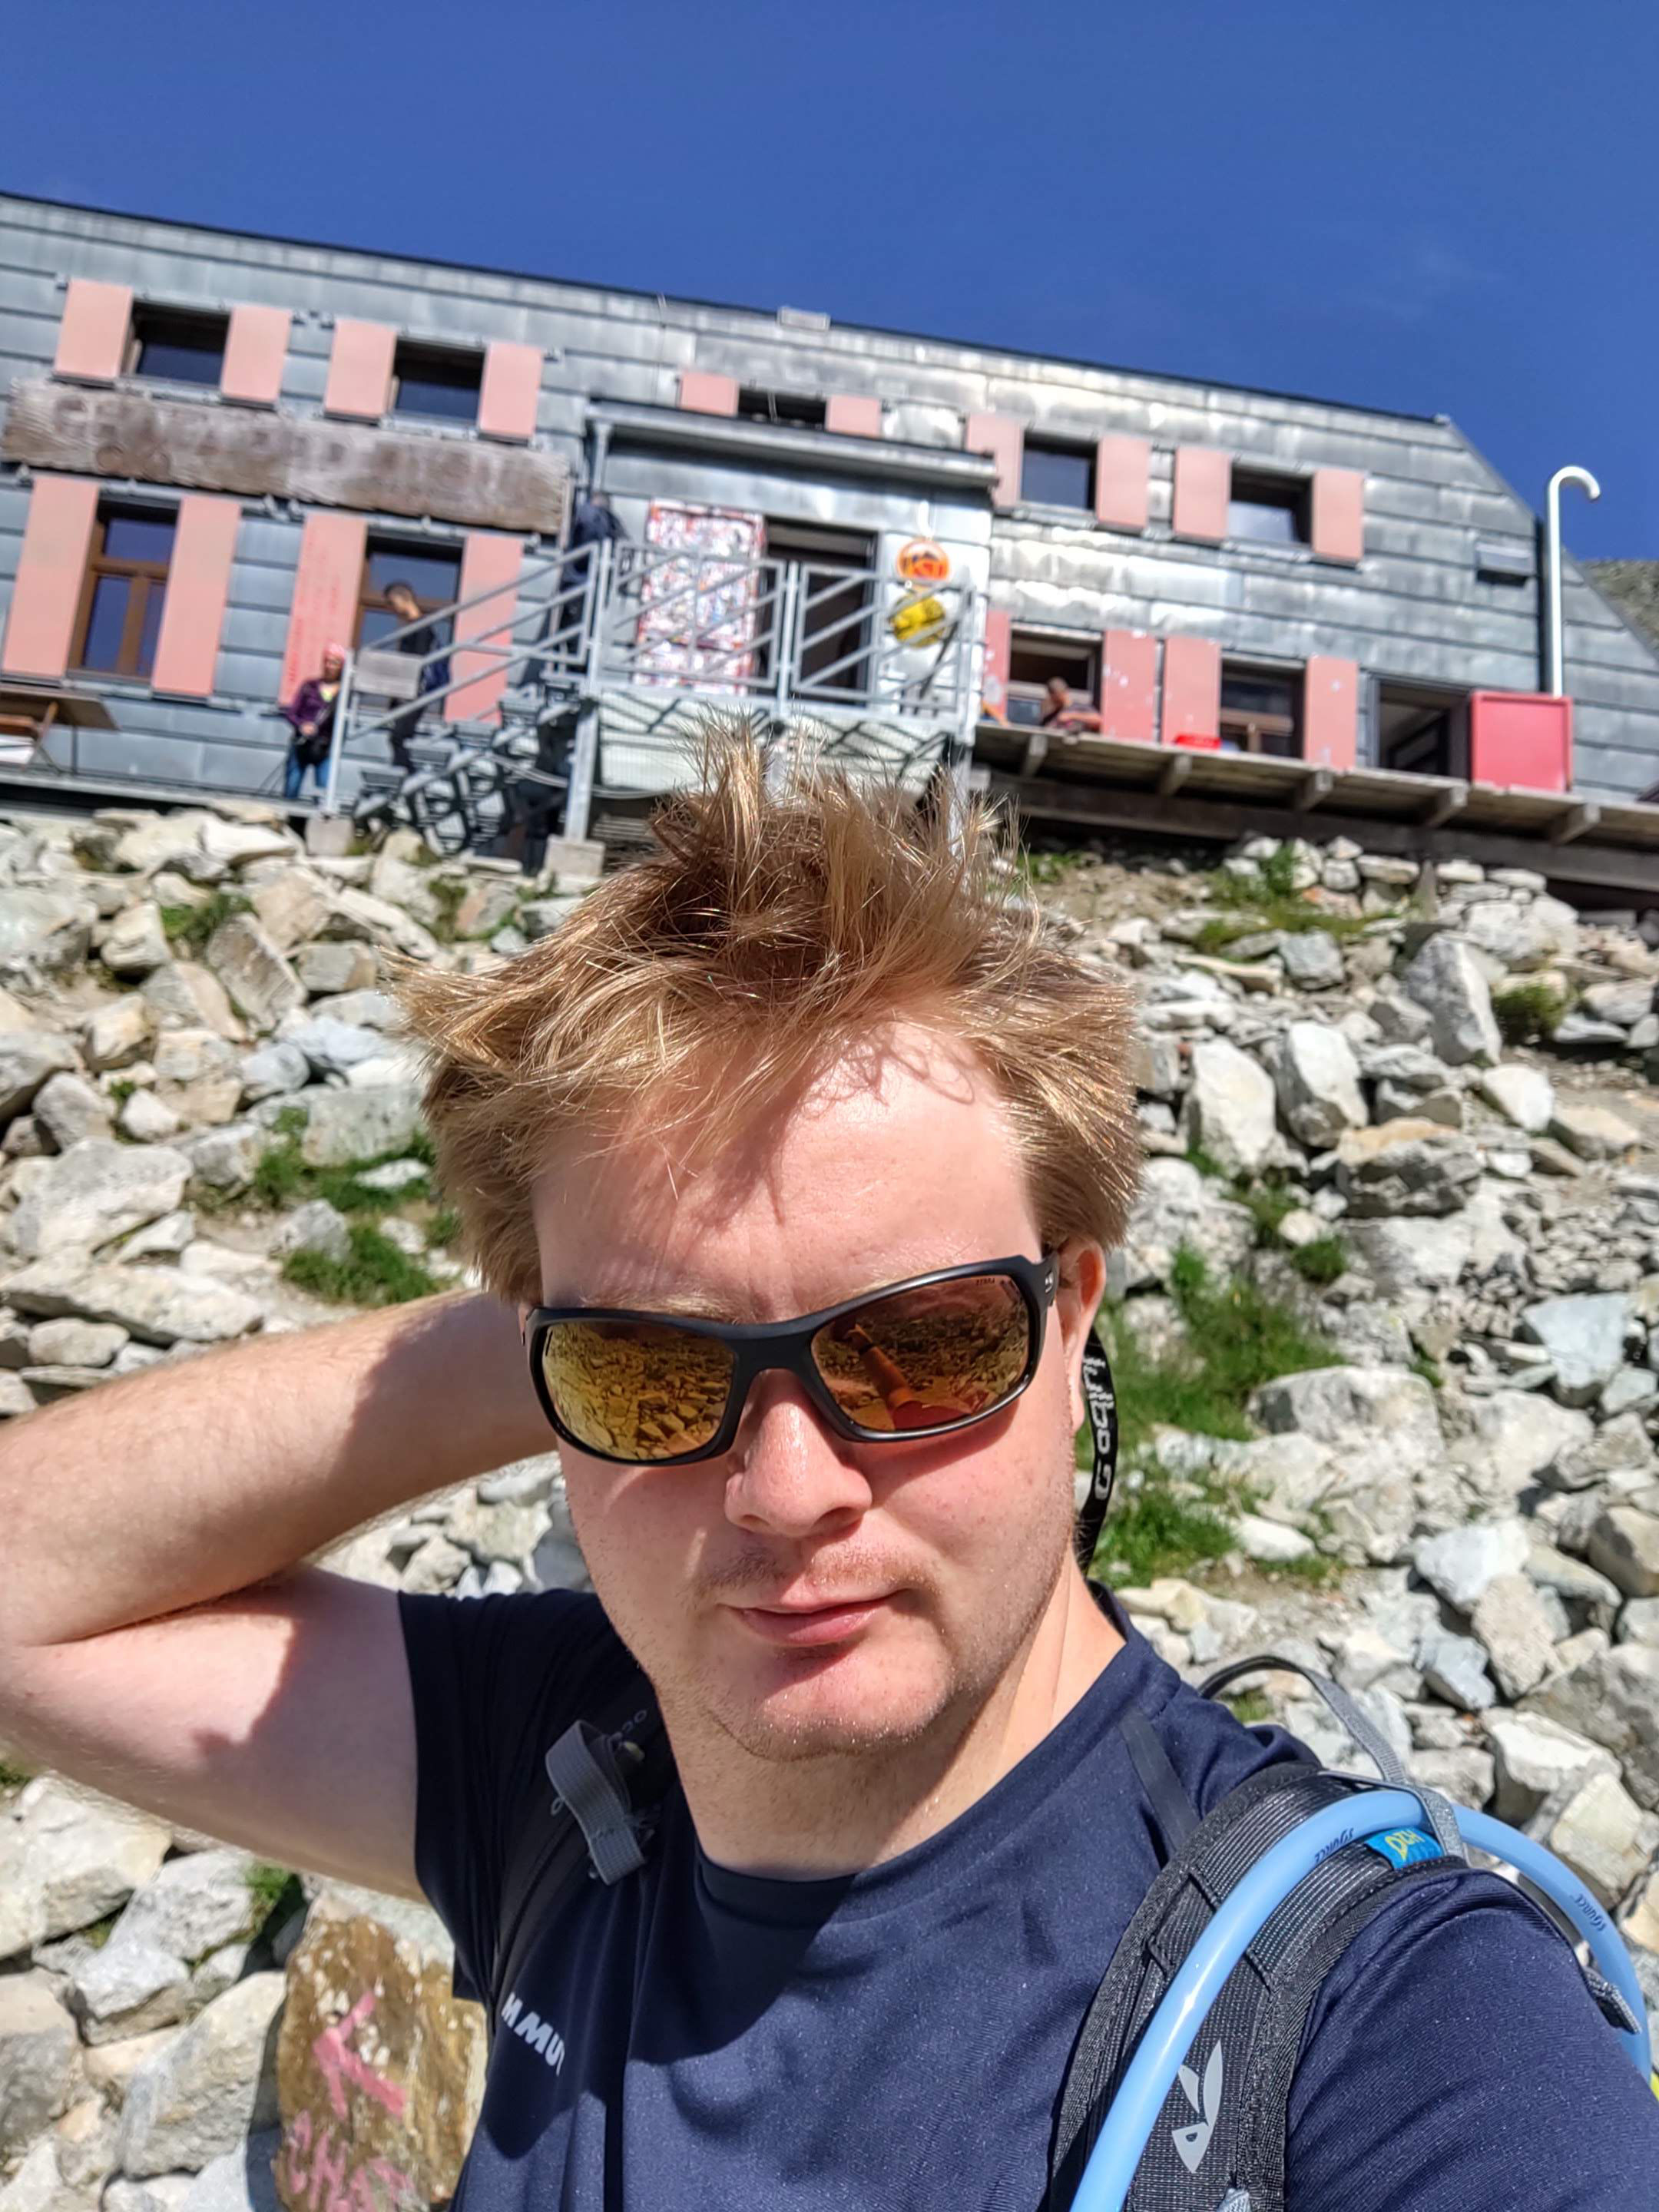
\includegraphics[scale=0.1]{../images/me2.jpg}}

\url{michal.nand@gmail.com}

\url{https://github.com/michalnand/}

 
\end{frame}


\end{document}
